\chapter{Discussion}

In this Chapter, we put together the final experiment results of all the network models presented in this thesis, and provide analysis over the results.

Table \ref{table:my-label1} records the performance of the neural network models on POS and NER. The POS performance is measured on the Penn Treebank data set, and the NER performance is measured on the CoNLL 2003 data set. It also includes the results from the state-of-the-art models on POS and NER. While our implementations obtain slightly lower accuracy score and F1 score than the state-of-art results, we emphasize that our main goal of this thesis is to compare different neural networks, and to present to new multi-task models.

Table \ref{table:my-label2} records the average decoding speed of different neural network models on the Penn Treebank and CoNLL 2003 test data. All experiments are conducted on a GPU. It's obvious that the less features used in the same model the faster the decoding speed of the model will be. In general, the greedy tagging systems using feedforward models are faster then the systems using BiLSTM models. Since the CRF based models introduce a transition matrix and uses dynamic programming algorithm to decode the sequence, they are slower than the systems without the CRF layer.

\begin{table}[]
\centering
\caption{Neural Network Models Accuracy and F1 Score}
\label{table:my-label1}
\begin{tabular}{|c|c|c|}
\hline
Model         & Penn Treebank (Accuracy)  & CoNLL 2003 (F1 Score)       \\ \hline
Syntaxnet    & \textbf{97.44}         &   _     \\ \hline
NeuroNet    & _    & \textbf{90.5}                \\ \hline 
Feedforward-word    & 95.89          &   84.12     \\ \hline
Feedforward-history & 97.28     & 86.54        \\ \hline
Feedforward-CRF     & 97.30          &   87.85     \\ \hline
BiLSTM  & 96.04     & 84.78                             \\ \hline
BiLSTM-Char & 97.21 & 88.32             \\ \hline
BiLSTM-Char-CRF & 97.34  & 90.11             \\ \hline
Feedforward-Mention2Vec  & _    & 88.97                       \\ \hline
BPE-Mention2Vec & 96.04     &  _   \\ \hline   
\end{tabular}
\end{table}

\begin{table}[]
\centering
\caption{Neural Network Models Decoding Speed}
\label{table:my-label2}
\begin{tabular}{|c|c|c|}
\hline
Model & Penn Treebank (words/sec) & CoNLL 2003 (words/sec) \\ \hline
Feedforward-word    & 30967    & 26819    \\ \hline
Feedforward-history & 19474    & 17609     \\ \hline
Feedforward-CRF     & 17877    & 17412     \\ \hline
BiLSTM              & 23036    & 20740       \\ \hline
BiLSTM-Char         & 13992    & 11271           \\ \hline
BiLSTM-Char-CRF     & 9009     & 10100        \\ \hline
Feedforward-Mention2Vec     & _      & 13445              \\ \hline
BPE-Mention2Vec     & 4923  &  _               \\ \hline   
\end{tabular}
\end{table}

Figure \ref{fig:pos} illustrates the trade-off between performance and decoding speed in POS systems using different neural network models. Among the neural network models for POS systems, BiLSTM-Char-CRF achieves the best per word accuracy 97.34\%, and Feedforward-CRF obtains the second best per word accuracy 97.30\%. Feedforward model achieves the fastest decoding speed since it employs a simple neural network without extra features: the POS greedy system using the Feedforward model decodes 1319 sentences per second. The line in Figure \ref{fig:pos} connects the BiLSTM-Char-CRF model which is the most accurate model and the Feedforward model which is the fastest model. The models above the line are faster but performs slightly worse than BiLSTM-Char-CRF, such as Feedforward-CRF and BiLSTM-Char. Models below the line such as BPE-Mention2Vec are slower and less accurate, which makes them less ideal for POS. Feedforward-History model is the fastest model with competitive performance on POS, and it is about 2 times faster than BiLSTM-Char-CRF.

Figure \ref{fig:ner} illustrates the trade-off between performance and speed of using different neural network models on CoNLL 2003. BiLSTM-Char-CRF achieves the highest F1 Score 90.11, and Feedforward-Mention2Vec obtains the second best F1 Score 88.79. Feedforward achieves the fastest decoding speed since it employs a simple neural network with no extra features: the NER greedy system using the Feedforward model decodes 2177 sentences per second. The line in Figure \ref{fig:ner} connects the BiLSTM-Char-CRF model which is the most accurate model and the Feedforward model which is the fastest model. The models above the line are faster but perform slightly worse than BiLSTM-Char-CRF, such as Feedforward-CRF and Feedforward-Mention2Vec. Models below the line are slower and less accurate, which makes them less ideal for NER. Feedforward-Mention2Vec model is the fastest model with competitive performance. Feedforward-Mention2Vec obtains 88.79 F1 score which is close to the best performance, and it is 1.3 times faster than the fully structured BiLSTM model.

As illustrated in Figure \ref{fig:pos} and Figure \ref{fig:ner}, the greedy sequence tagging systems using feedforward networks can achieve comparable performance and faster speed than the systems using recurrent models on POS; the multi-task model (Feedforward-Mention2Vec) performs competitively with the state-of-the-art model (BiLSTM-Char-CRF) on NER.

Table \ref{table:my-label3} compares the performance and speed of BiLSTM-Char-CRF and Feedforward-Mention2Vec on CoNLL 2003 and OntoNotes. It shows that Feedforward-Mention2Vec with a simple architecture can achieve competitive performance with BiLSTM-Char-CRF on CoNLL 2003 and OntoNotes. The speed gap between Feedforward-Mention2Vec and BiLSTM-Char-CRF grows as the number of named entity types increases. There is more speed benefit in using a multi-task model like Feedforward-Mention2Vec when there are more types to classify.

\begin{table}[]
\centering
\caption{F1 Scores and Decoding Speed on CoNLL 2003 and OntoNotes }
\label{table:my-label3}
\begin{tabular}{|c|c|c|c|c|}
\hline
& \multicolumn{2}{c|}{F1 Score} & \multicolumn{2}{c|}{Decoding Speed (Words/Sec)} \\ \hline
& CoNLL 2003     & OntoNotes    & CoNLL 2003              & OntoNotes             \\ \hline
Feedforward-Mention2Vec & 88.97          & 86.34        & 13445                   & 10812                 \\ \hline
BiLSTM-Char-CRF         & 90.11          & 83.18        & 10100                   & 7667                  \\ \hline
\end{tabular}
\end{table}

\begin{figure}
  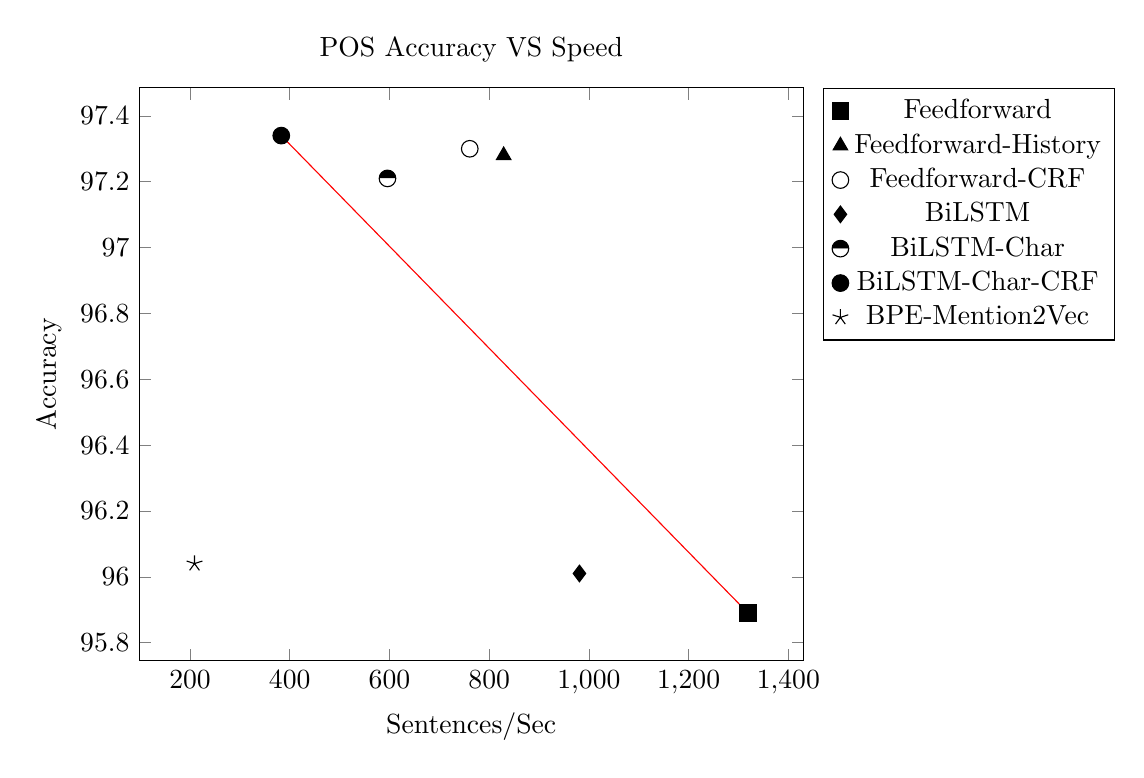
\begin{tikzpicture}
	\begin{axis}[%
	ylabel={Accuracy},
	xlabel={Sentences/Sec},
	scale only axis,
	mark size=3.0pt,
	title={POS Accuracy VS Speed},
	scatter/classes={%
		Feedforward={mark=square*},%
		Feedforward-History={mark=triangle*},%
		Feedforward-CRF={mark=o,draw=black},%
		BiLSTM={mark=diamond*},%
		BiLSTM-Char={mark=halfcircle*},%
		BiLSTM-Char-CRF={mark=otimes*},%
		BPE-Mention2Vec={mark=star}},%
	legend style={at={(1.03,1)},anchor=north west,draw=black,fill=white,align=left}]
	\addplot[scatter,only marks,%
		scatter src=explicit symbolic]%
	table[meta=label] {
    x     y      label
    1319  95.89   Feedforward 
    829   97.28   Feedforward-History 
    761   97.30   Feedforward-CRF 
    981   96.01   BiLSTM 
    596   97.21   BiLSTM-Char
    383   97.34   BiLSTM-Char-CRF
    209   96.04   BPE-Mention2Vec
    };
    \addplot+ [mark=none]table {
    x     y      label
    1319   95.89   Feedforward  
    383   97.34   BiLSTM-Char-CRF
    
    };
	\addlegendentry{Feedforward}
	\addlegendentry{Feedforward-History}
	\addlegendentry{Feedforward-CRF}
	\addlegendentry{BiLSTM}
	\addlegendentry{BiLSTM-Char}
	\addlegendentry{BiLSTM-Char-CRF}
	\addlegendentry{BPE-Mention2Vec}
	\end{axis}
\end{tikzpicture}
 \caption{Results of the POS system using different Neural Network Models}
  \label{fig:pos}
\end{figure}

\begin{figure}
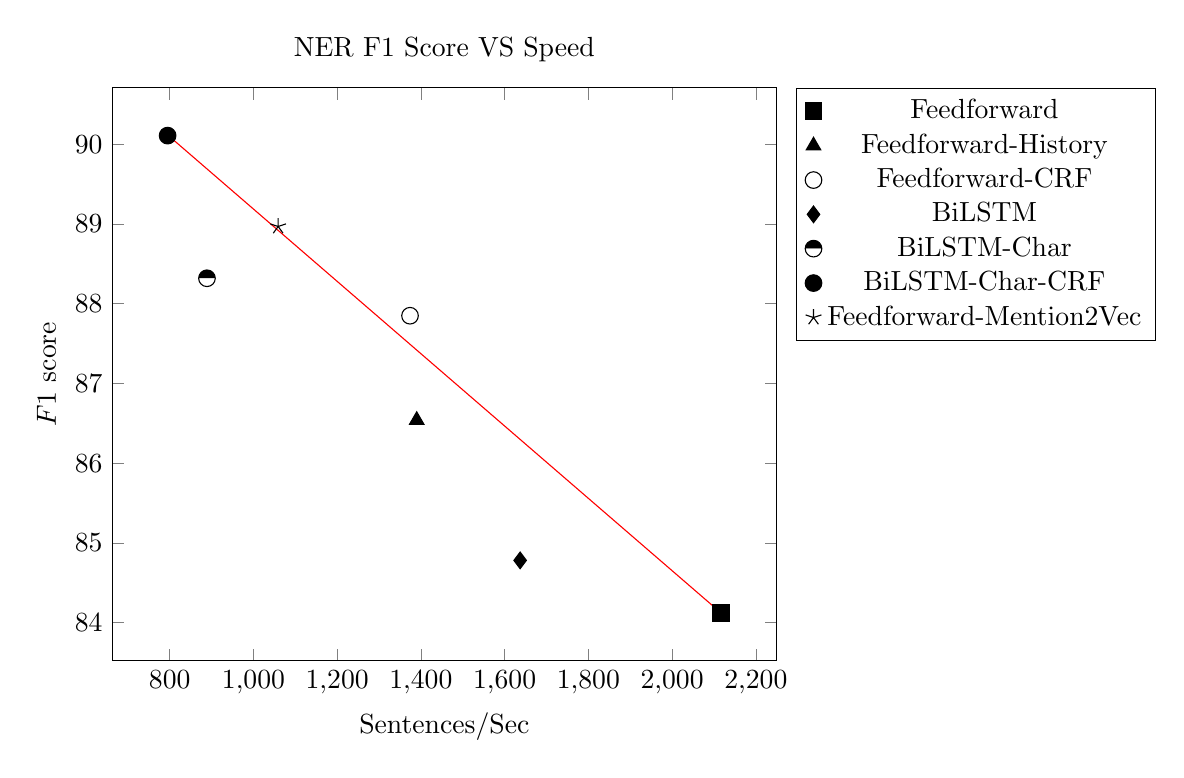
\begin{tikzpicture}
	\begin{axis}[%
	ylabel={$F1$ score},
	xlabel={Sentences/Sec},
	scale only axis,
	mark size=3.0pt,
	title={NER F1 Score VS Speed},
	scatter/classes={%
		Feedforward={mark=square*},%
		Feedforward-History={mark=triangle*},%
		Feedforward-CRF={mark=o,draw=black},%
		BiLSTM={mark=diamond*},%
		BiLSTM-Char={mark=halfcircle*},%
		BiLSTM-Char-CRF={mark=otimes*},%
		Feedforward-Mention2Vec={mark=star}},%
	legend style={at={(1.03,1)},anchor=north west,draw=black,fill=white,align=left}]
	\addplot[scatter,only marks,%
		scatter src=explicit symbolic]%
	table[meta=label] {
    x     y      label
    2117   84.12   Feedforward 
    1390   86.54   Feedforward-History 
    1374   87.85   Feedforward-CRF 
    1637   84.78   BiLSTM 
    889   88.32    BiLSTM-Char
    795   90.11    BiLSTM-Char-CRF
    1059   88.97   Feedforward-Mention2Vec
	};
	\addplot+ [mark=none]table {
    x     y      label
    2117   84.12   Feedforward 
    797   90.11   BiLSTM-Char-CRF
    
    };
	\addlegendentry{Feedforward}
	\addlegendentry{Feedforward-History}
	\addlegendentry{Feedforward-CRF}
	\addlegendentry{BiLSTM}
	\addlegendentry{BiLSTM-Char}
	\addlegendentry{BiLSTM-Char-CRF}
	\addlegendentry{Feedforward-Mention2Vec}
	\end{axis}
\end{tikzpicture}
 \caption{Results of the NER system using different Neural Network Models}
  \label{fig:ner}
\end{figure}

